\section{Durchführung}
\label{sec:Durchführung}
\subsection{Aufbau}
Zuerst muss der Versuch aufgebaut werden. Dazu wird an den Tank eine Kreuzung K1 angebracht. An beide Abzweige dieser Kreuzung wird ein Sperrventil V1/V2
montiert und dann das Nadelventil bzw. ein Schlauch S1. An dem letzten Ausgang der Kreuzung K1 kommt ein T-Stück T1. An diesen Abzweig wird die Kaltkathode
angebracht. Der letzte Ausgang von T1 geht in ein weiteres T-Stück T2, an dem die Glühkathode und hinter einem Sperrventil V3 die Turbopumpe angebracht sind.
An den Ausgang der Turbopumpe wird ein Sperrventil V4 und eine Kreuzung K2 montiert. An die Kreuzung K2 wird das andere Ende des Schlauches S1 angebracht. An K2
wird ebenfalls ein T-Stück T3 montiert, an dem das digitale und das analoge Pirani-Vakuummeter montiert sind. Am letzten Abzweig von K2 wird der Schlauch S2 und
damit die Drehschieberpumpe angebracht. Bei jedem Flansch ist darauf zu achten, dass ein passender Dichtungsring eingesetzt wird. Dieser Aufbau ist auch
nochmal in den Abbildungen \ref{img:ab1},\ref{img:ab2} und \ref{img:ab3} dokumentiert.
\begin{figure}
	\centering
	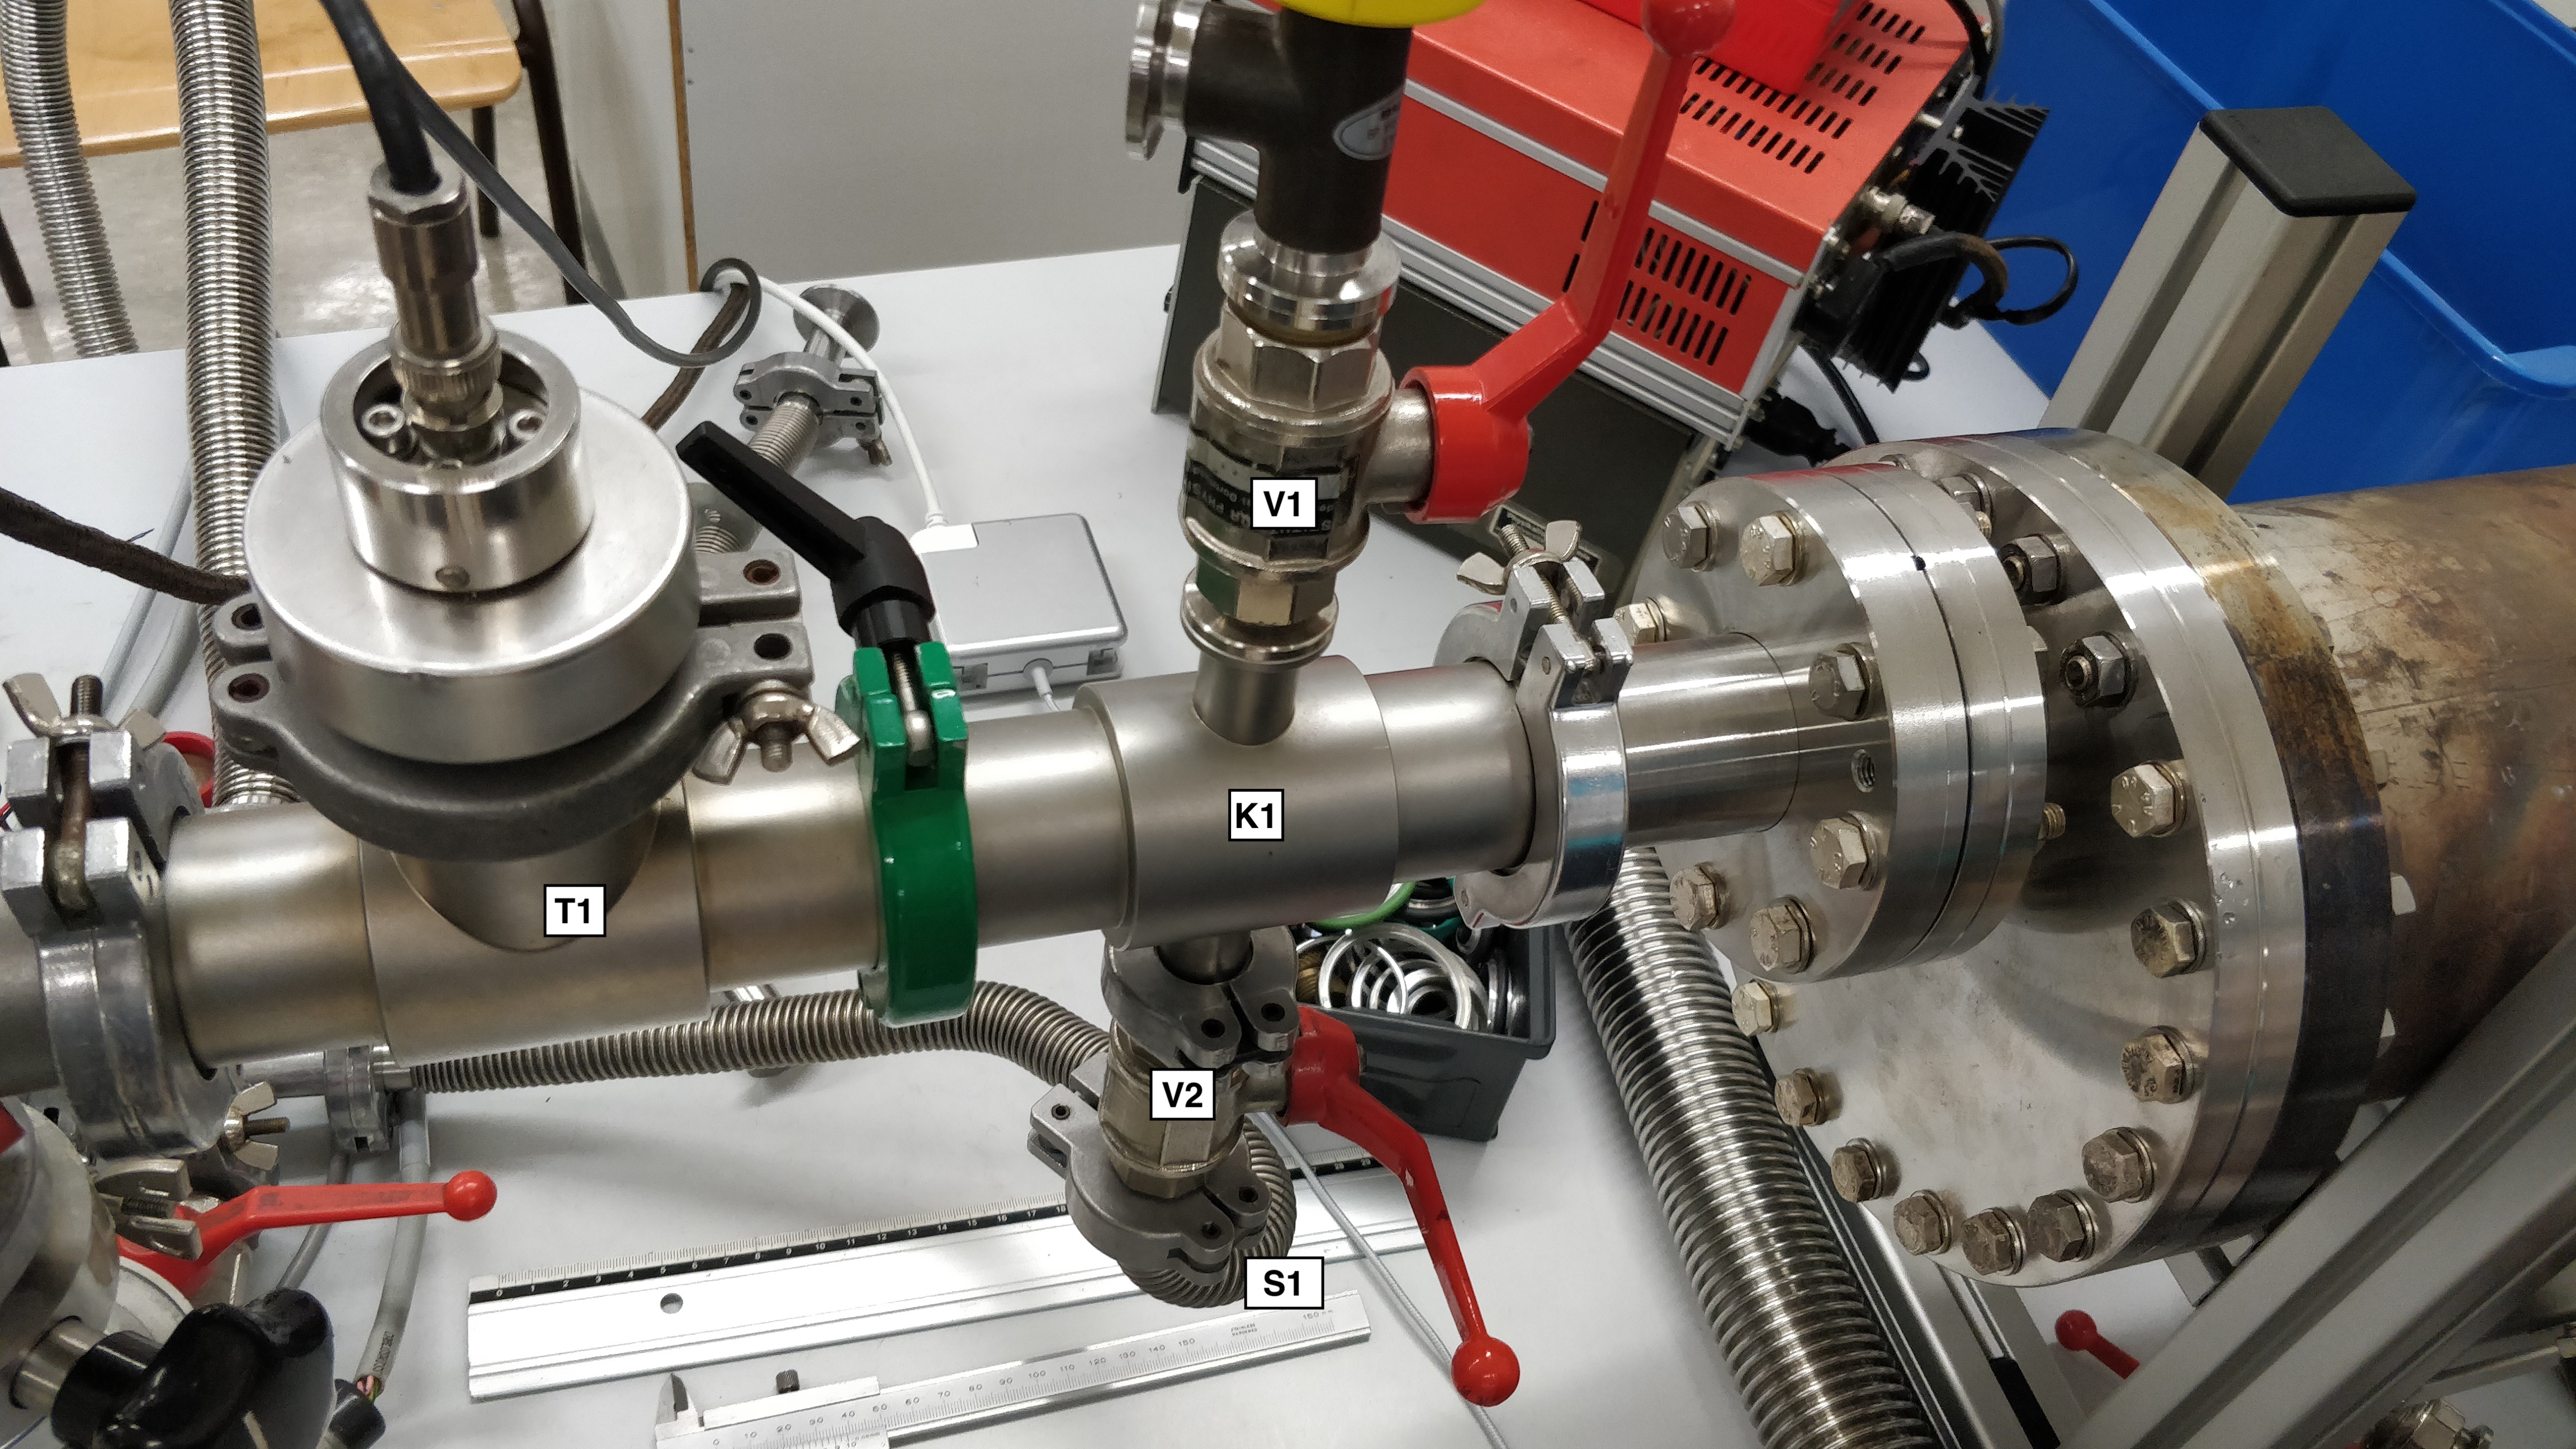
\includegraphics[width=0.8\textwidth]{img/Aufbau1.jpg}
	\caption{Erste Ansicht des Aufbaus.}
	\label{img:ab1}
\end{figure}
\begin{figure}
	\centering
	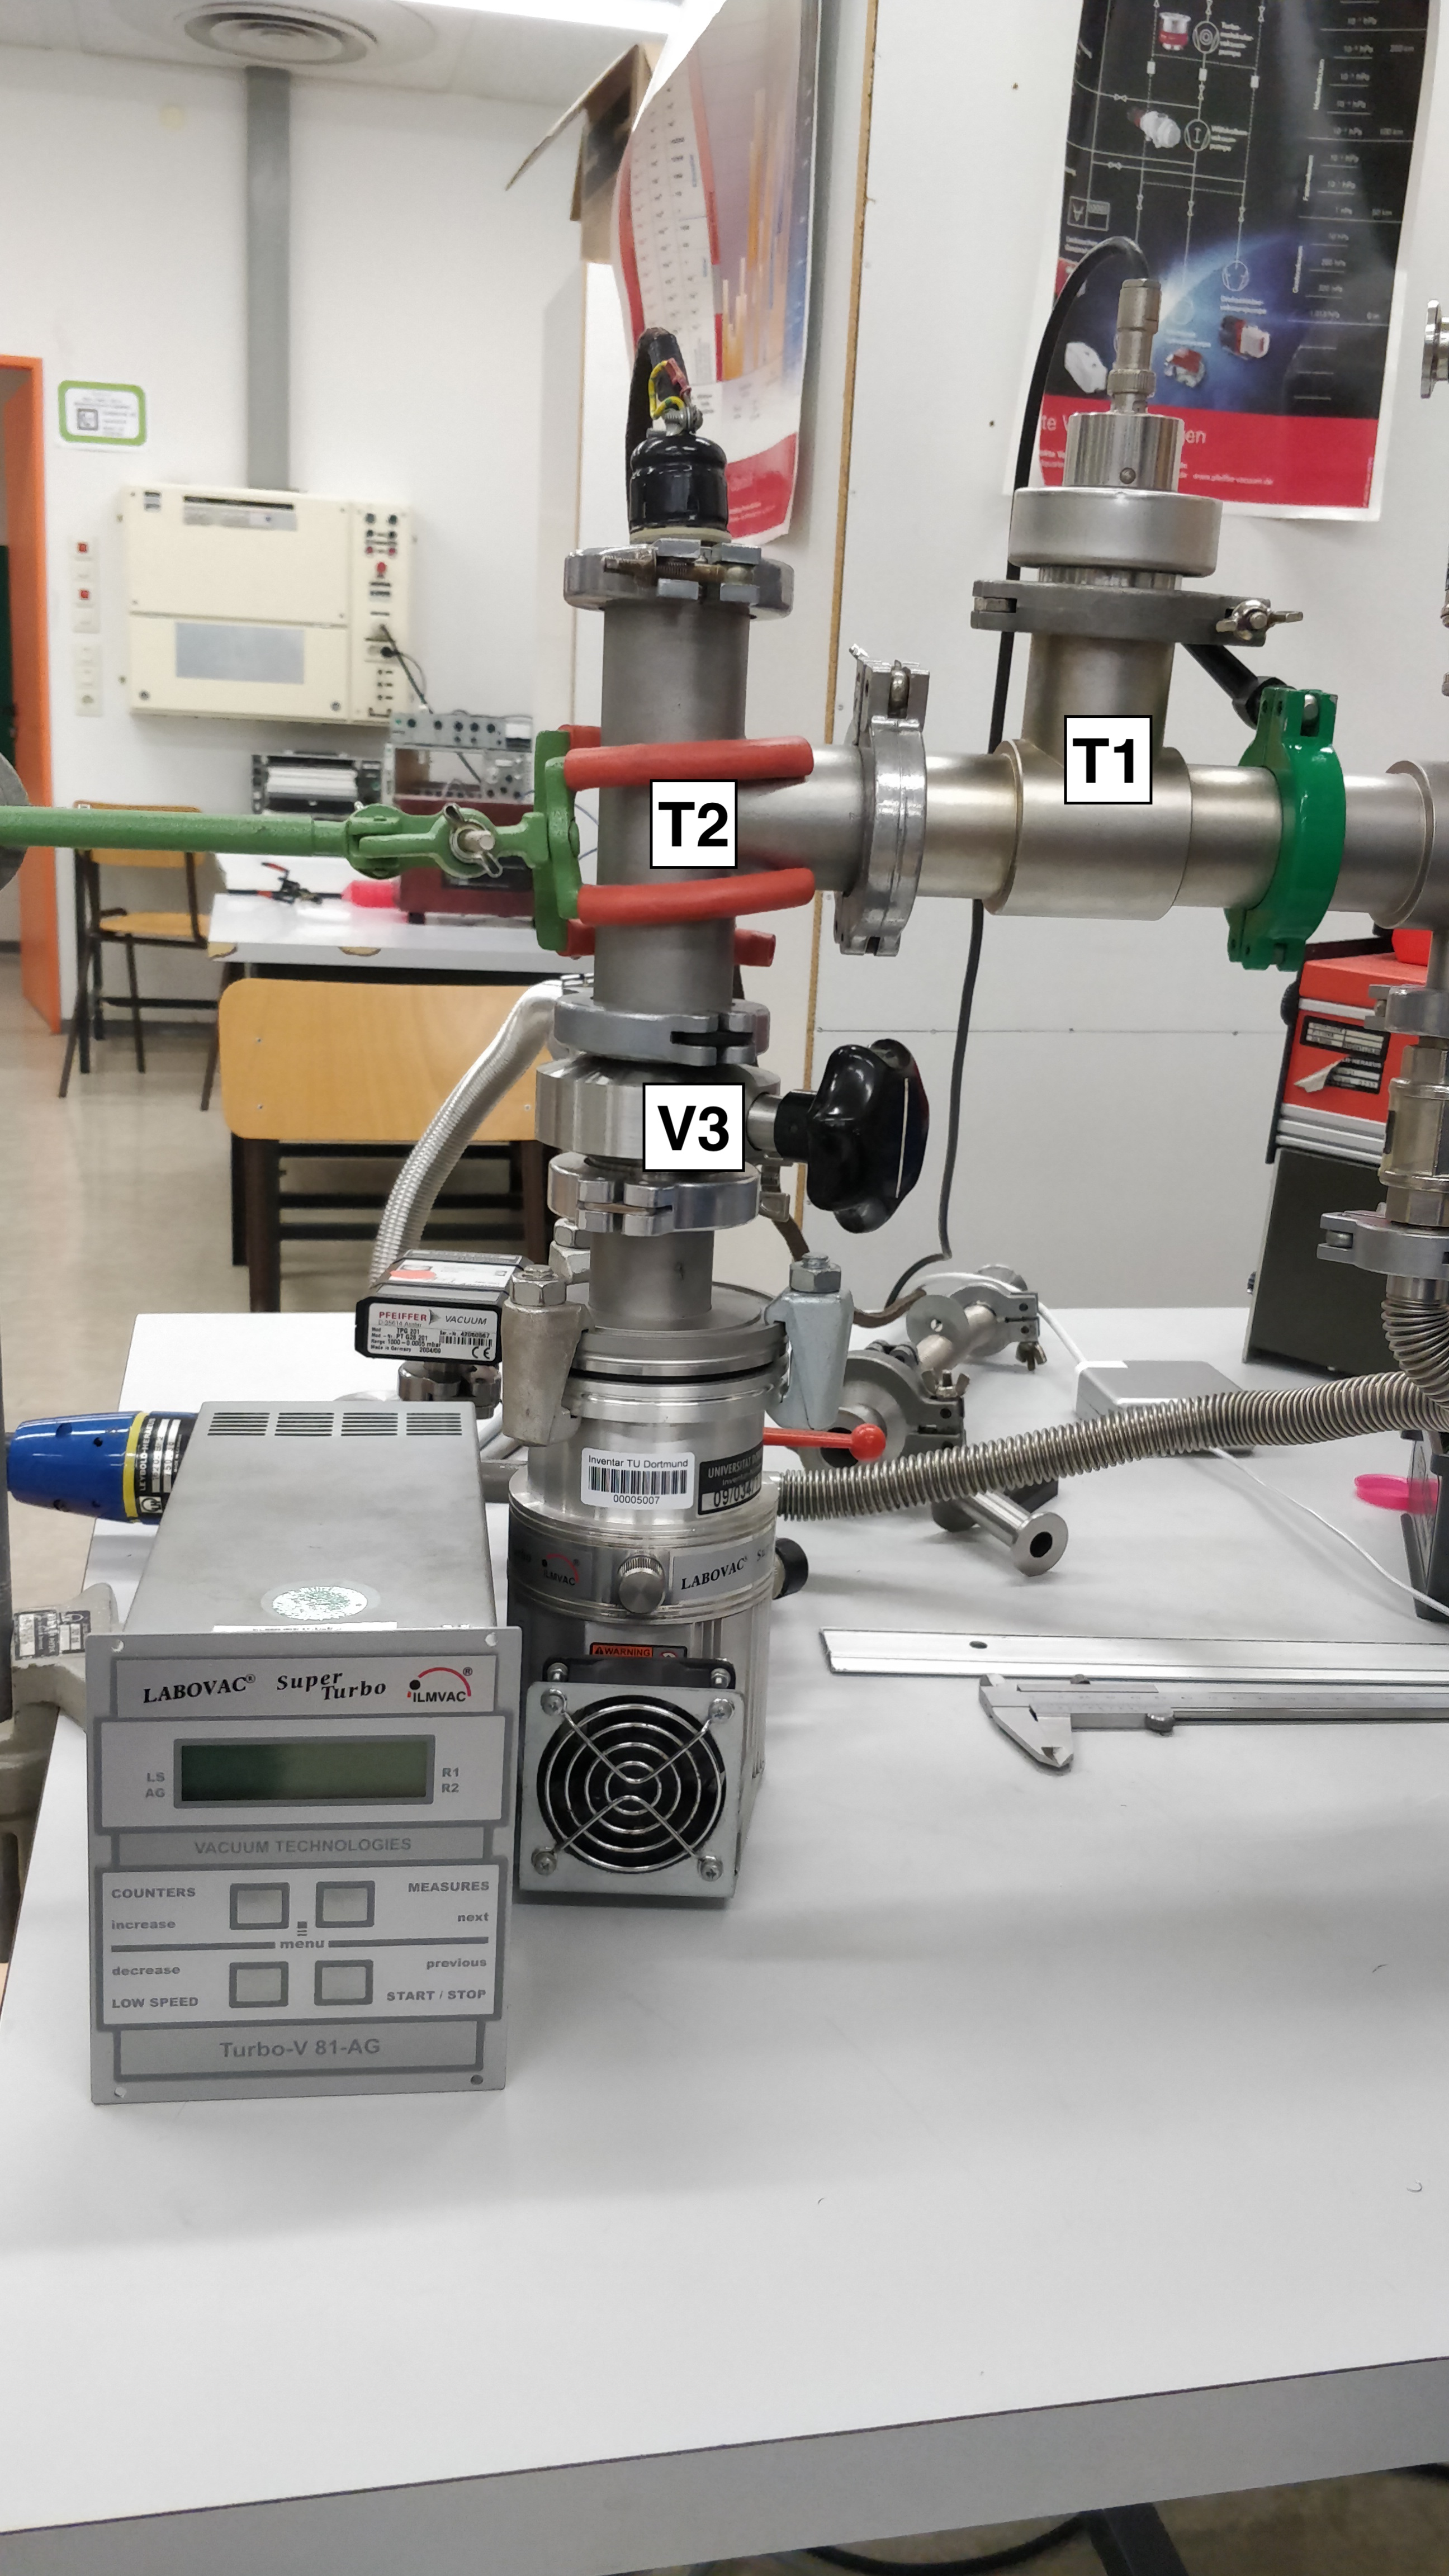
\includegraphics[width=0.8\textwidth]{img/Aufbau2.jpg}
	\caption{Zweite Ansicht des Aufbaus.}
	\label{img:ab2}
\end{figure}
\begin{figure}
	\centering
	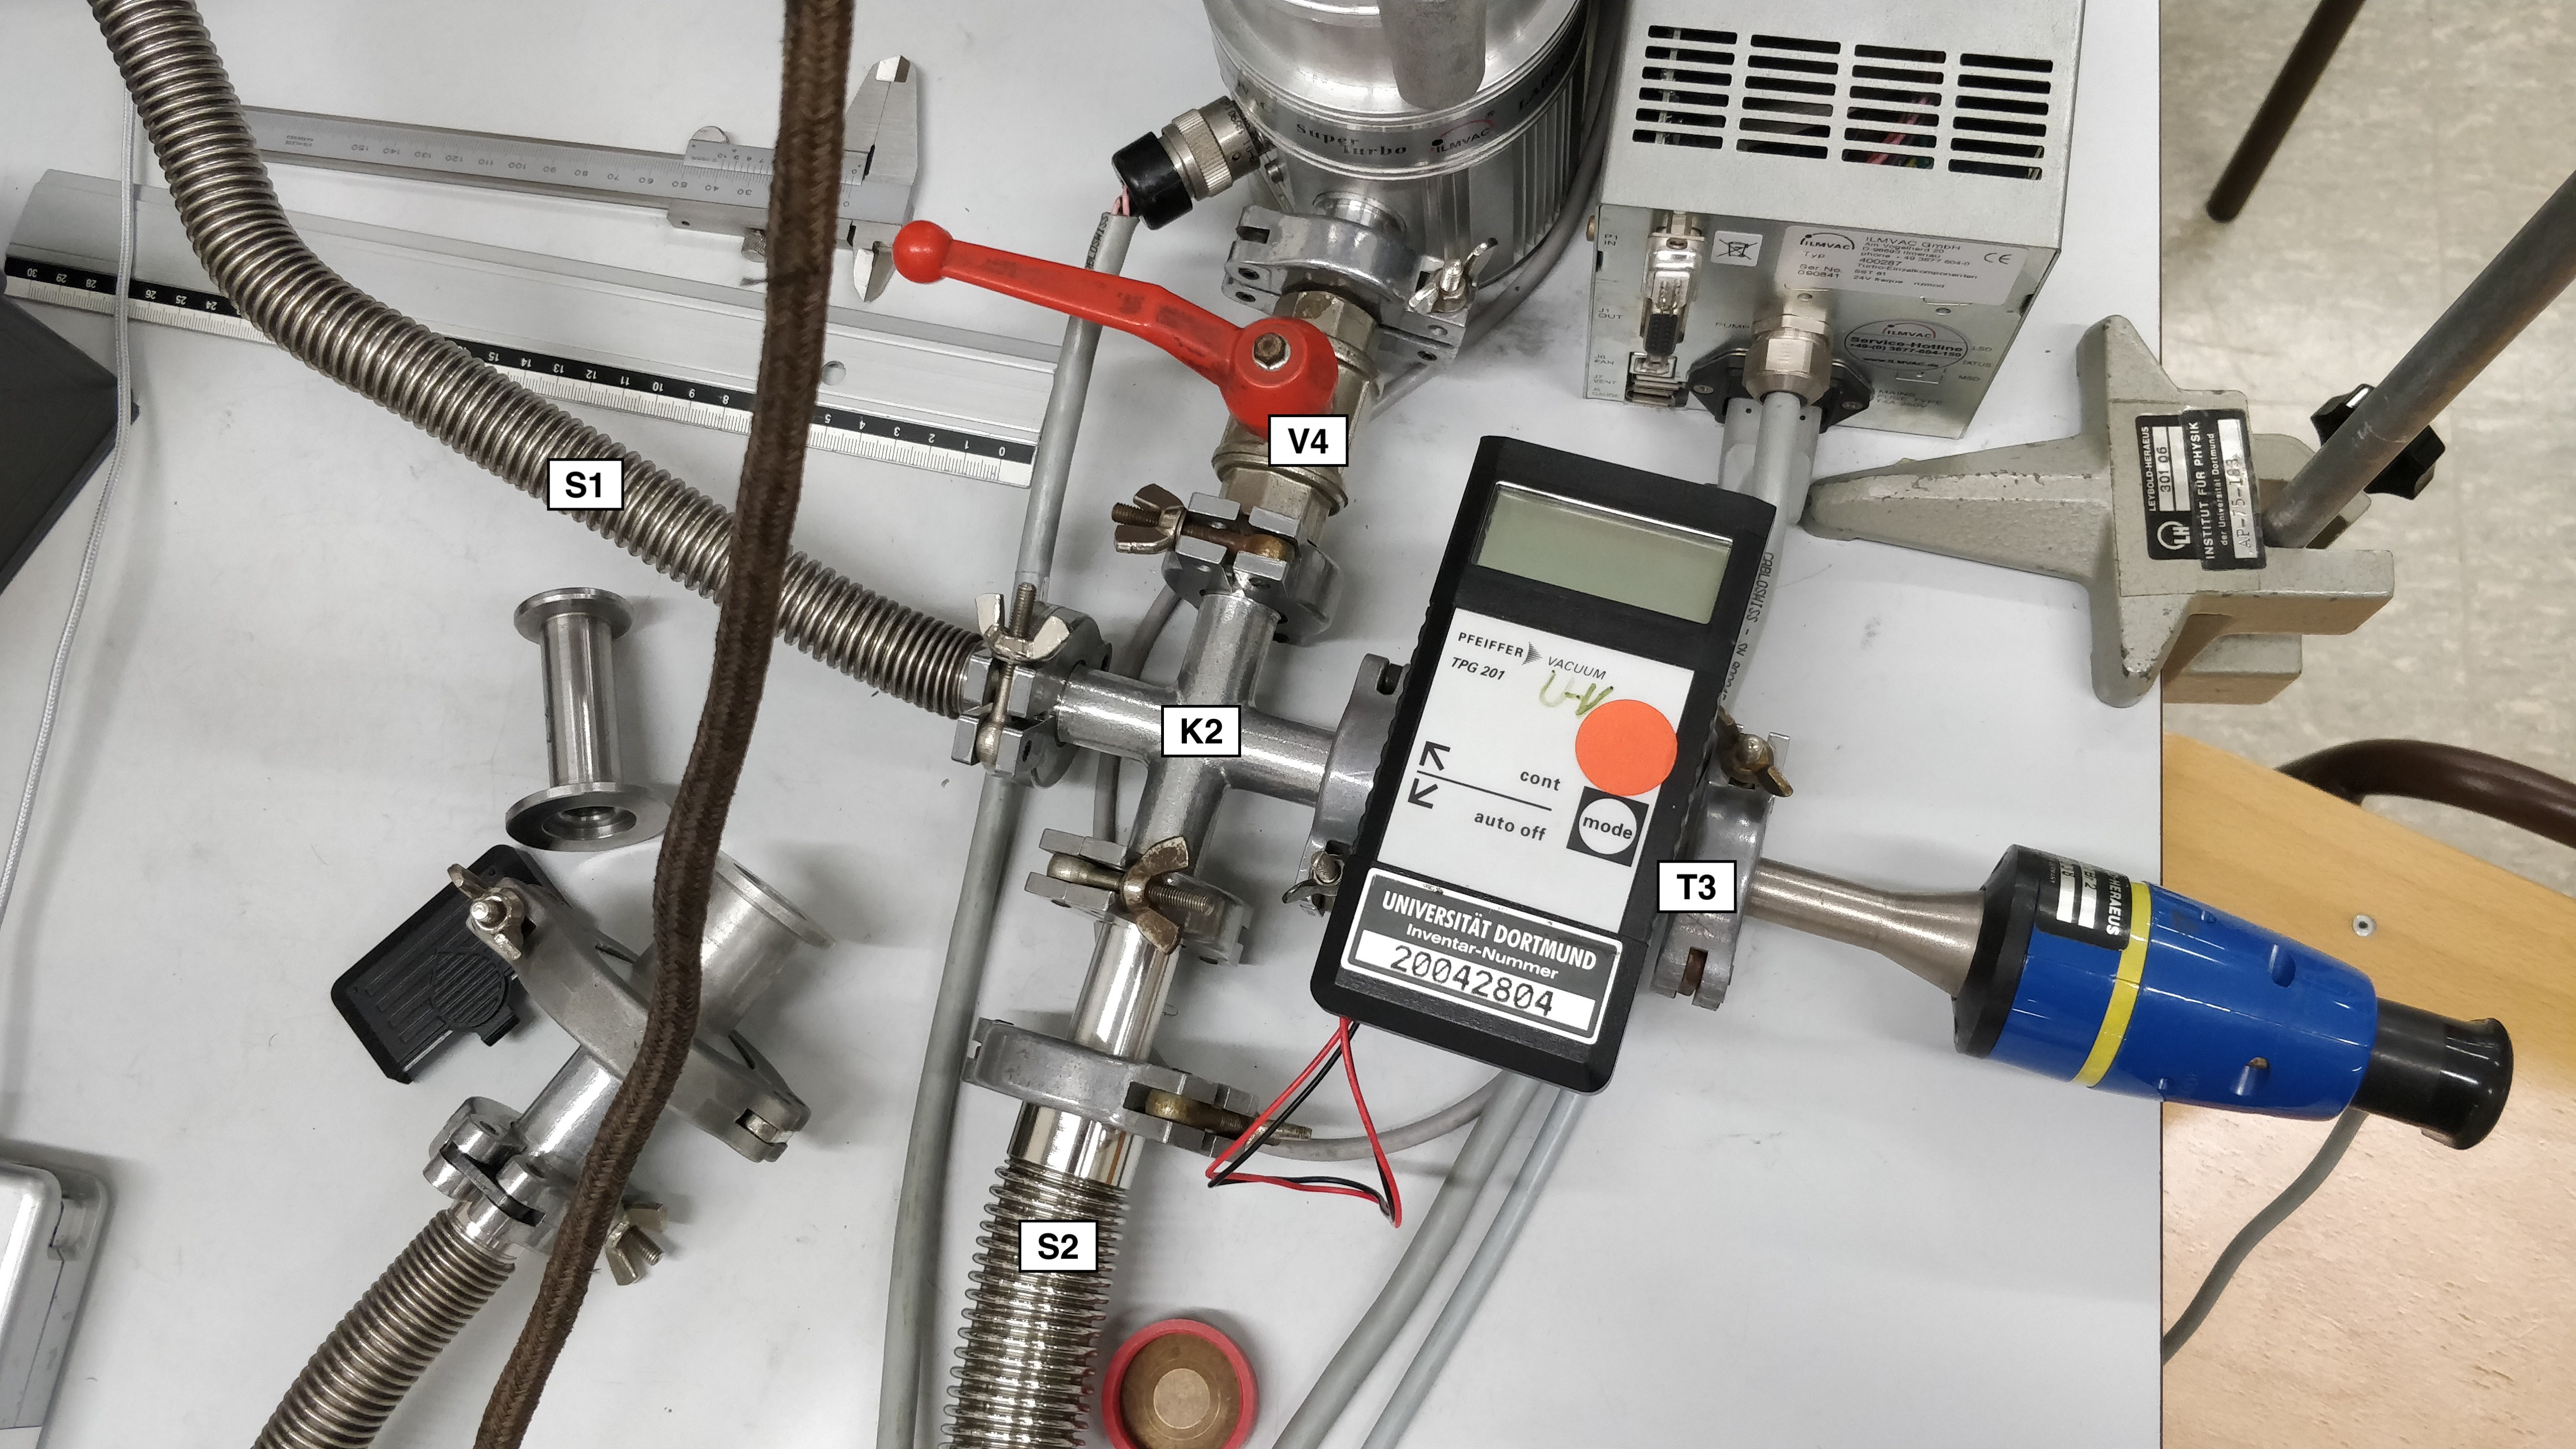
\includegraphics[width=0.8\textwidth]{img/Aufbau3.jpg}
	\caption{Erste Ansicht des Aufbaus.}
	\label{img:ab3}
\end{figure}
\subsection{Messprogramm}
Zuerst wir der Aufbau überprüft. Dazu wird die Drehschieberpumpe angeschaltet und der Druck vermessen. nach wenigen Minuten sollte er auf
$\SI{0.03}{\milli \bar}$ abgefallen sein. Zusätzlich kann jetzt die Turbopumpe verwendet werden, um Ablagerungen abzupumpen. Nun wird der Aufbau wieder für das
eigentliche Messprogramm belüftet.

Es werden beide Pumpen mit zwei Messmethoden vermessen. Zuerst werden die Ventile so eingestellt, das nur die
Drehschieberpumpe am Tank angeschlossen ist. Dann wird der Druck im Tank gegen die Pumpzeit aufgenommen. Es soll bis zu einem Endruck von
$\SI{0.04}{\milli \bar}$ gepumpt werden. Diese Messung wird fünfmal wiederholt. Es ist zu empfehlen, nicht in festen Zeitintervallen den Druck aufzunehmen,
sondern zu gut ablesbaren Drücken die Zeit aufzunehmen.
Die zweite Methode ist die Leckratenmessung. Dabei wird am Nadelventil ein Leck eingestellt, sodass sich bei laufender Pumpe ein Druckgleichgewicht einstellt.
Dann wird das Ventil an der Pumpe geschlossen, und der Druckanstieg gegen die Zeit wird aufgenommen. Es wird über eine Größenordnung gemessen. Diese Messung
wird für vier Gleichgewichtsdrücke jeweils dreimal wiederholt. Als Gleichgewichtsdrücke eignen sich $\SI{0.1}{\milli \bar}$,
$\SI{0.4}{\milli \bar}$, $\SI{0.8}{\milli \bar}$ und $\SI{1}{\milli \bar}$. Wenn der Aufbau
hinreichend evakuiert ist, werden die Ventile so eingestellt, dass die Turbopumpe am Tank angeschlossen ist und die Drehschieberpumpe nur am Ausgang der
Turbopumpe angeschlossen ist. So wird der Aufbau auf $\SI{5e-5}{\milli \bar}$ abgepumpt. Jetzt wird mit dem Nadelventil der Aufbau auf $\SI{5e-3}{\milli \bar}$
belüftet und der analog zur Drehschieberpumpe die Evakuierungskurve aufgenommen. Die Leckratenmessung ist ebenfalls analog zur Drehschieberpumpe mit den
Gleichgewichtsdrücken $\SI{5e-5}{\milli \bar}$, $\SI{10e-5}{\milli \bar}$, $\SI{15e-5}{\milli \bar}$ und $\SI{20e-5}{\milli \bar}$.

Zuletzt muss noch das Volumen bestimmt werden. Dazu wird der Aufbau belüftet und demontiert. Die Volumen der einzelnen Teile werden dann nachgeschlagen oder
gemessen.
